\section{Problem description and analysis}
\label{sec:Problem}

\subsection{Problem description}
A shared risk link group (SRLG) is a group of links that share a component whose failure causes the failure of all links in the group. A link can belong to multiple SRLGs.

An example of such a component is the fiber conduit \cite{bhandari1994optimal} in optical networks, where several optical links may be placed side-by-side in one single conduit, as illustrated in Fig.\ref{fig:SRLGgraph}. Links (1,2), (3,2) and (3,4) are placed inside a single conduit, while links (3,2) and (3,4) also share another single conduit. If a conduit gets cut, the corresponding links will fail. Each conduit corresponds a SRLG.  Other example applications of SRLGs are the correlated congestion of transportation networks and cascading failures of power grid networks \cite{coudert2007shared}.
\begin{figure}[htbp]

  \centering
\subfigure[Physical topology with conduit]{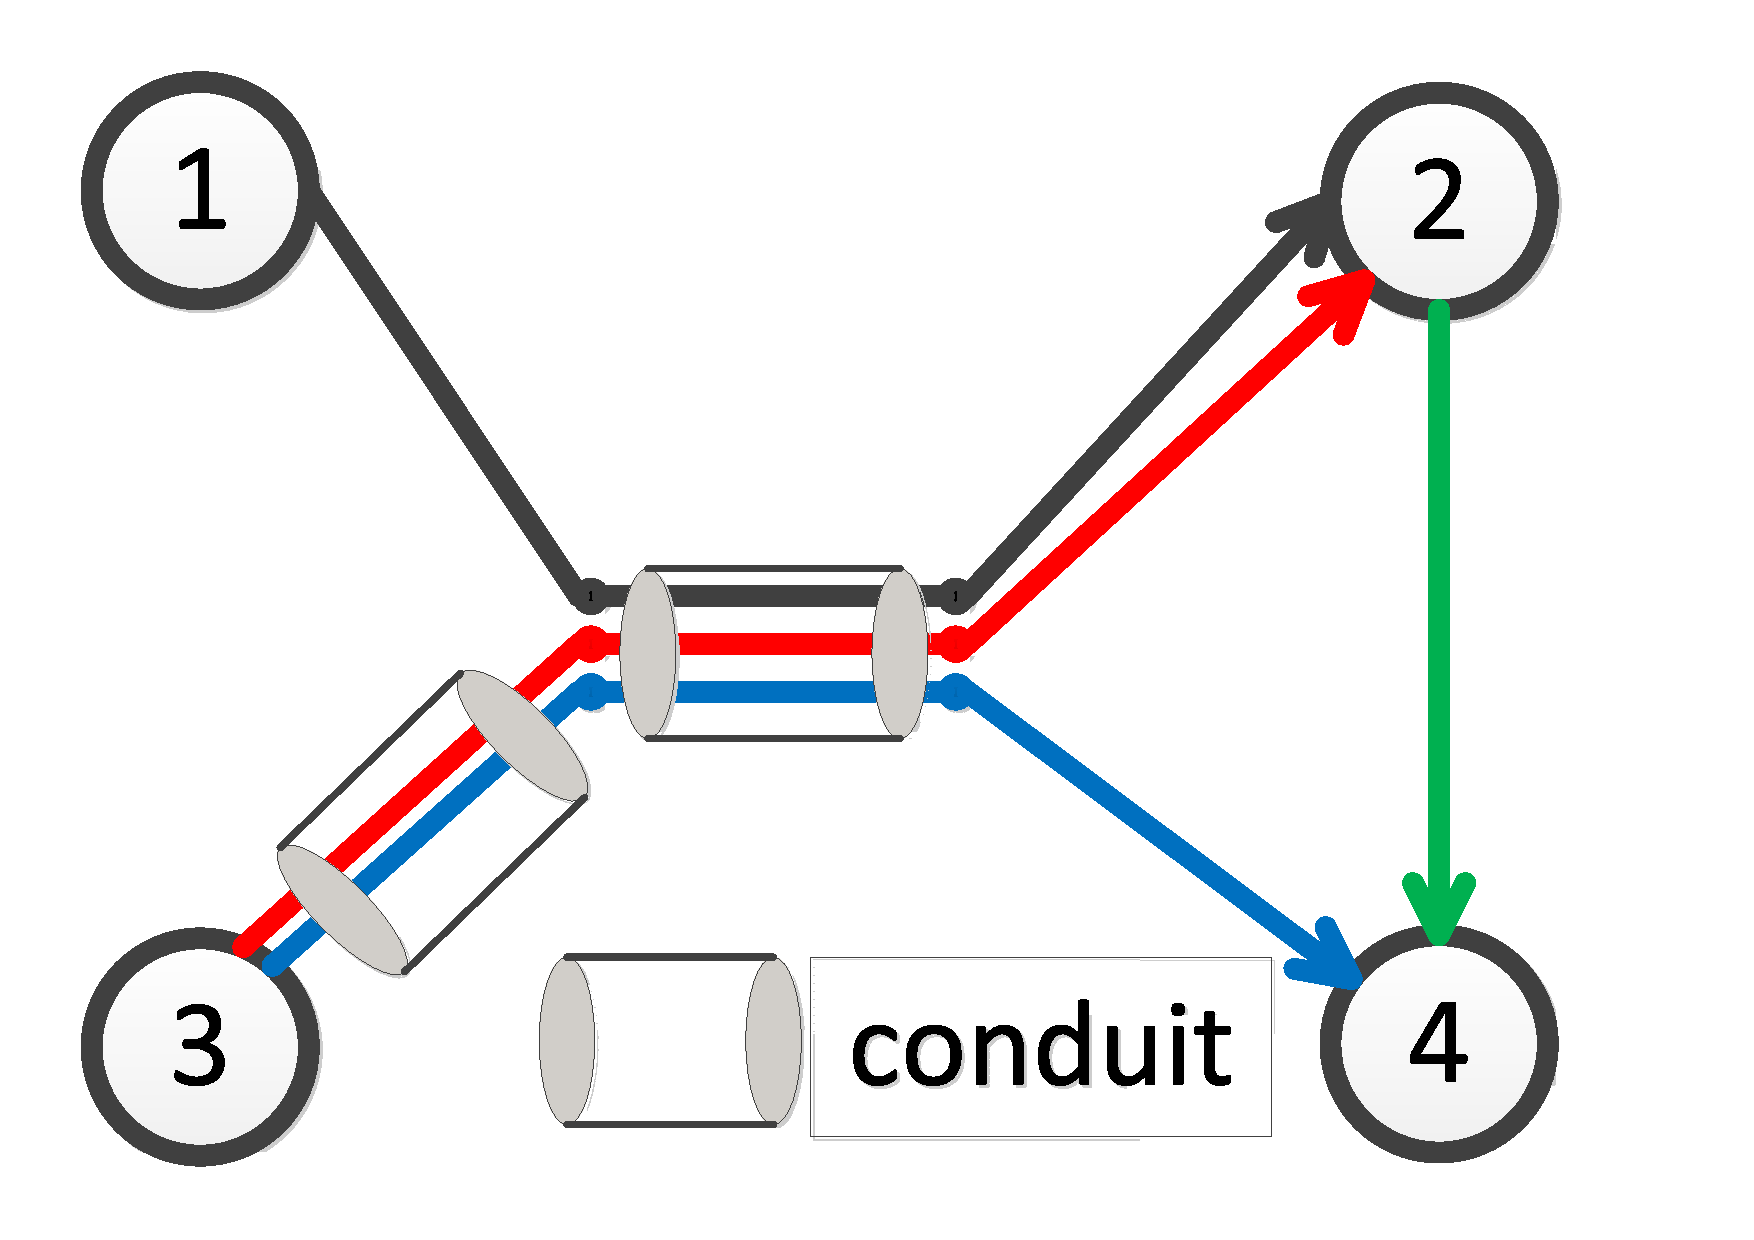
\includegraphics[width=1.25 in]{franz/PhysicalGraph}
}
\subfigure[Network Graph]{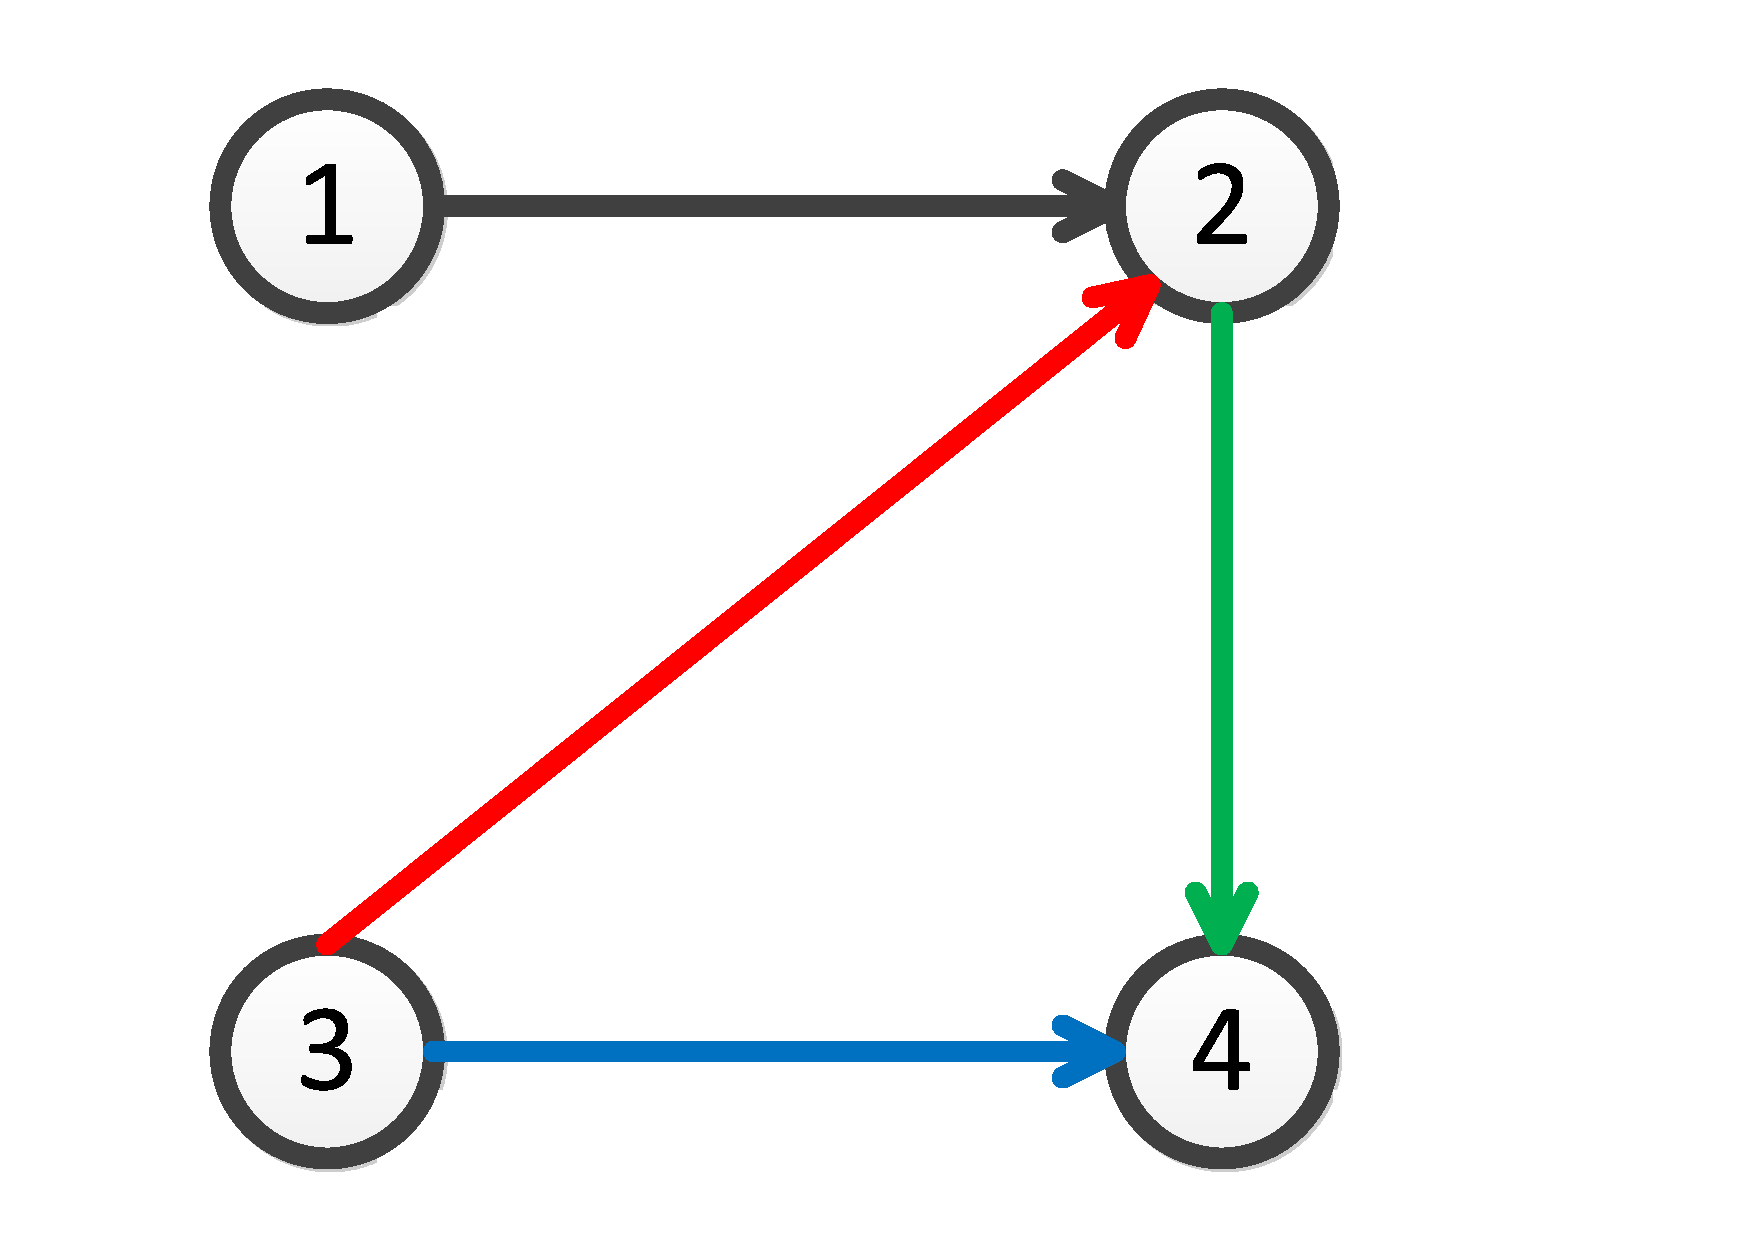
\includegraphics[width=0.9 in]{franz/VirtualGraph}
}
\caption{Example of shared risk link group(SRLG)}\label{fig:SRLGgraph}
\label{fig:Logic shift operation}

\end{figure}

Let $\mathbb{R}$ be the risk (failure) set in the network. Each risk may correspond to a conduit cut, a fiber cut, a card failure at a node, a software failure, or any combination of these factors. For $r_i \in \mathbb{R}$, its SRLG is the link set associated with risk $r_i$, denoted as $\mathbb{R}_{r_i}$, where $1\leq i\leq \chi$ and $\chi=|{\mathbb{R}}|$ is the number of risks/SRLGs.  In Fig.\ref{fig:CompositeGraph}(a), the network includes five SRLGs $\mathbb{R}_{r_1}=\{e_1,e_9\}$, $\mathbb{R}_{r_2}=\{e_2,e_3,e_{19}\}$, $\mathbb{R}_{r_3}=\{e_2,e_4,e_{11},e_{17}\}$, $\mathbb{R}_{r_4}=\{e_5,e_{13}\}$, $\mathbb{R}_{r_5}=\{e_{15},e_{18}\}$. In this example, link $e_2$ is in two SRLGs $\mathbb{R}_{r_2}$ and $\mathbb{R}_{r_3}$.

A network is often represented as a graph $G(\mathbb{V},\mathbb{E})$, where $\mathbb{V}$ is the set of $|\mathbb{V}|$ nodes (which for instance represent routers) and $\mathbb{E}$ is the set of $|\mathbb{E}|$ links (which for instance represent optical fiber lines or radio channels). Links may be characterized by weights representing for instance their delay, length, or cost. For a link $e_i$, we denote the weight of the link as $w_{e_i}$. The weight of a path $P$ is denoted as $w_P=\sum\limits_{e_i\in \mathbb{P}}w_{e_i}$, which is the sum of  the weight of each link in the path.

Let $r_P$ denote the risk set that impacts a path $P$, that is $r_P=\{r\in \mathbb{R}$: path $P$ contains links in $\mathbb{R}_r\}$. In Fig.\ref{fig:CompositeGraph}(c), the link set on the AP is $\mathbb{AP}=\{e_1,e_2,e_3,e_4,e_5,e_6,e_7,e_8\}$ with $e_1\in \mathbb{R}_{r_1}$, $e_2\in \mathbb{R}_{r_2}$, $e_2\in \mathbb{R}_{r_3}$, $e_3\in \mathbb{R}_{r_2}$, $e_4\in \mathbb{R}_{r_3}$, $e_5\in \mathbb{R}_{r_4}$,  the risk set of AP is ${r}_{{AP}}=\{r_1, r_2, r_3, r_4\}$. $\mathbb{\mathbb{ER}}$ denotes the set of links not belonging to AP that share the common risks with AP. In Fig.\ref{fig:CompositeGraph}(c), $\mathbb{\mathbb{ER}}=\{e_9,e_{11},e_{17},e_{13},e_{19}\}$.

SRLG-disjoint paths share no common risks among themselves, that is, the failure of a path due to a risk would not affect other paths. Fig.\ref{fig:CompositeGraph}(b) shows two SRLG-disjoint paths, denoted as AP and BP. As these two paths share no common risk, if AP fails, BP can still work. This paper focuses on finding  two SRLG-disjoint paths for path protection, which can be described as follows.
%\revtao{review's advice: It was also mentioned that "For multiple SRLG-disjoint paths, the failure of a path due to a risk would not affect other paths", it would be nice to give an example using Fig. 3.}

\textbf{Min-Min SRLG-disjoint routing problem.} Given a graph $G(\mathbb{V},\mathbb{E})$, a weight $w_{e_i}$ associated with each link $e_i\in \mathbb{E}$, a source  $s$ and a destination  $d$,  find a pair of SRLG disjoint paths from $s$ to $d$ (denoted as $AP$ and $BP$), thus that  the smallest path weight of the two disjoint paths is minimized, that is,

\begin{equation}
\begin{array}{*{20}{c}}
   {\mathop {minimize}\limits_{AP,BP} } & {\min \left( {{w_{AP}},{w_{BP}}} \right)}  \\
   {subject\ to} & {{r_{AP}} \cap {r_{BP}}{\rm{ = }}\phi }  \\
   {} & {\mathbb{AP} \cap \mathbb{BP}{\rm{ = }}\phi }  \\
\end{array}
\label{eq:problem definition}
\end{equation}
where ${w_{AP}}$ and ${w_{BP}}$ are the path weights of AP and BP, respectively, $\mathbb{AP}$ and $\mathbb{BP}$ are the link sets on paths AP and BP, respectively, ${r_{AP}}$ and ${r_{BP}}$ are the risk sets that impacts AP and BP, respectively.

%\begin{figure*}[tp]
%\centering
%\begin{minipage}[t]{0.3\linewidth}
%\centering
%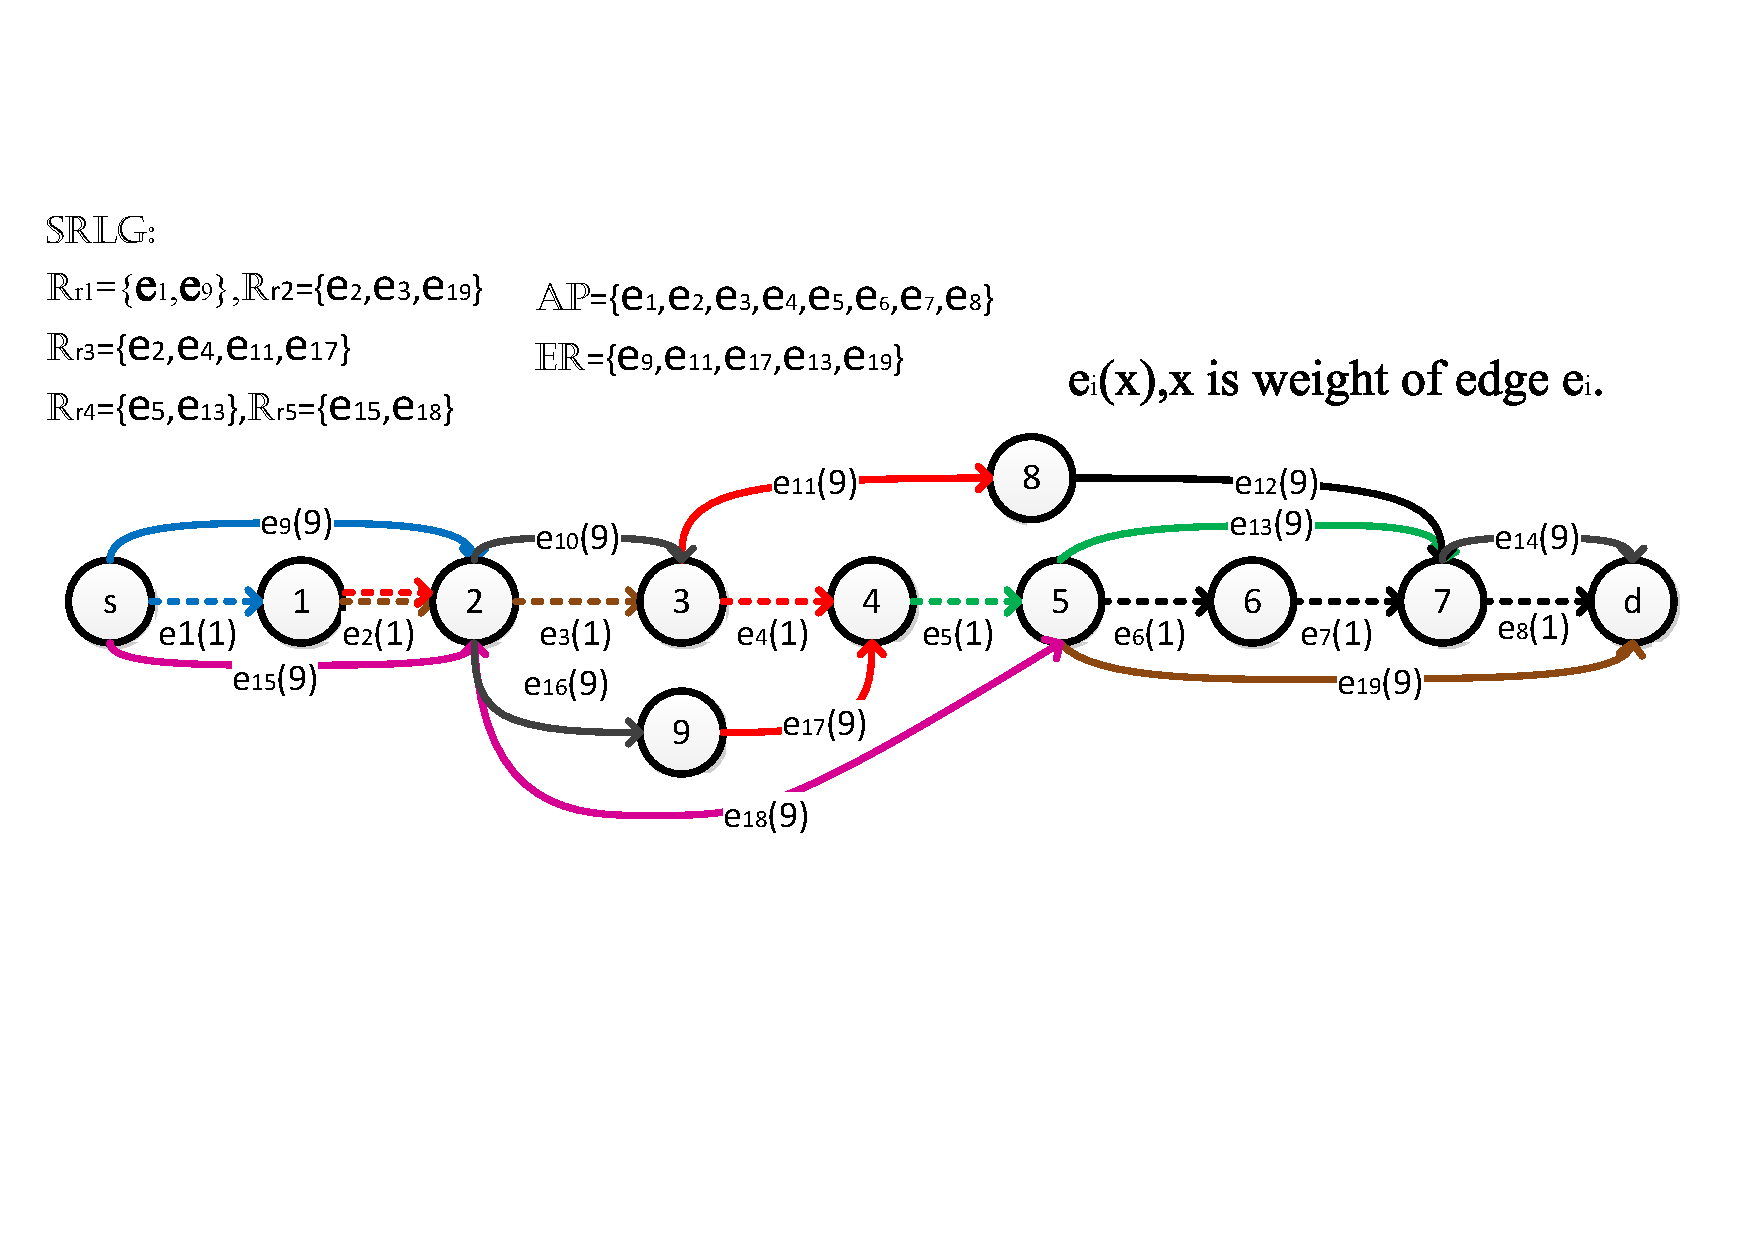
\includegraphics[width=3.5in]{franz/InitialGraph}
%\caption{$\mathbb{AP}=\{e_1,e_2,e_3,e_4,e_5,e_6,e_7,e_8\}$, $\mathbb{\mathbb{ER}}=\{e_9,e_{11},e_{17},e_{13},e_{19}\}$.  SRLGs: $\mathbb{R}_{r_1}=\{e_1,e_9\}$,$\mathbb{R}_{r_2}=\{e_2,e_3,e_{19}\}$,$\mathbb{R}_{r_3}=\{e_2,e_4,e_{11},e_{17}\}$,$\mathbb{R}_{r_4}=\{e_5,e_{13}\}$,$\mathbb{R}_{r_5}=\{e_{15},e_{18}\}$}
%\label{fig:Initial Graph}
%\end{minipage}
%\hfill
%\begin{minipage}[t]{0.3\linewidth}
%\centering
%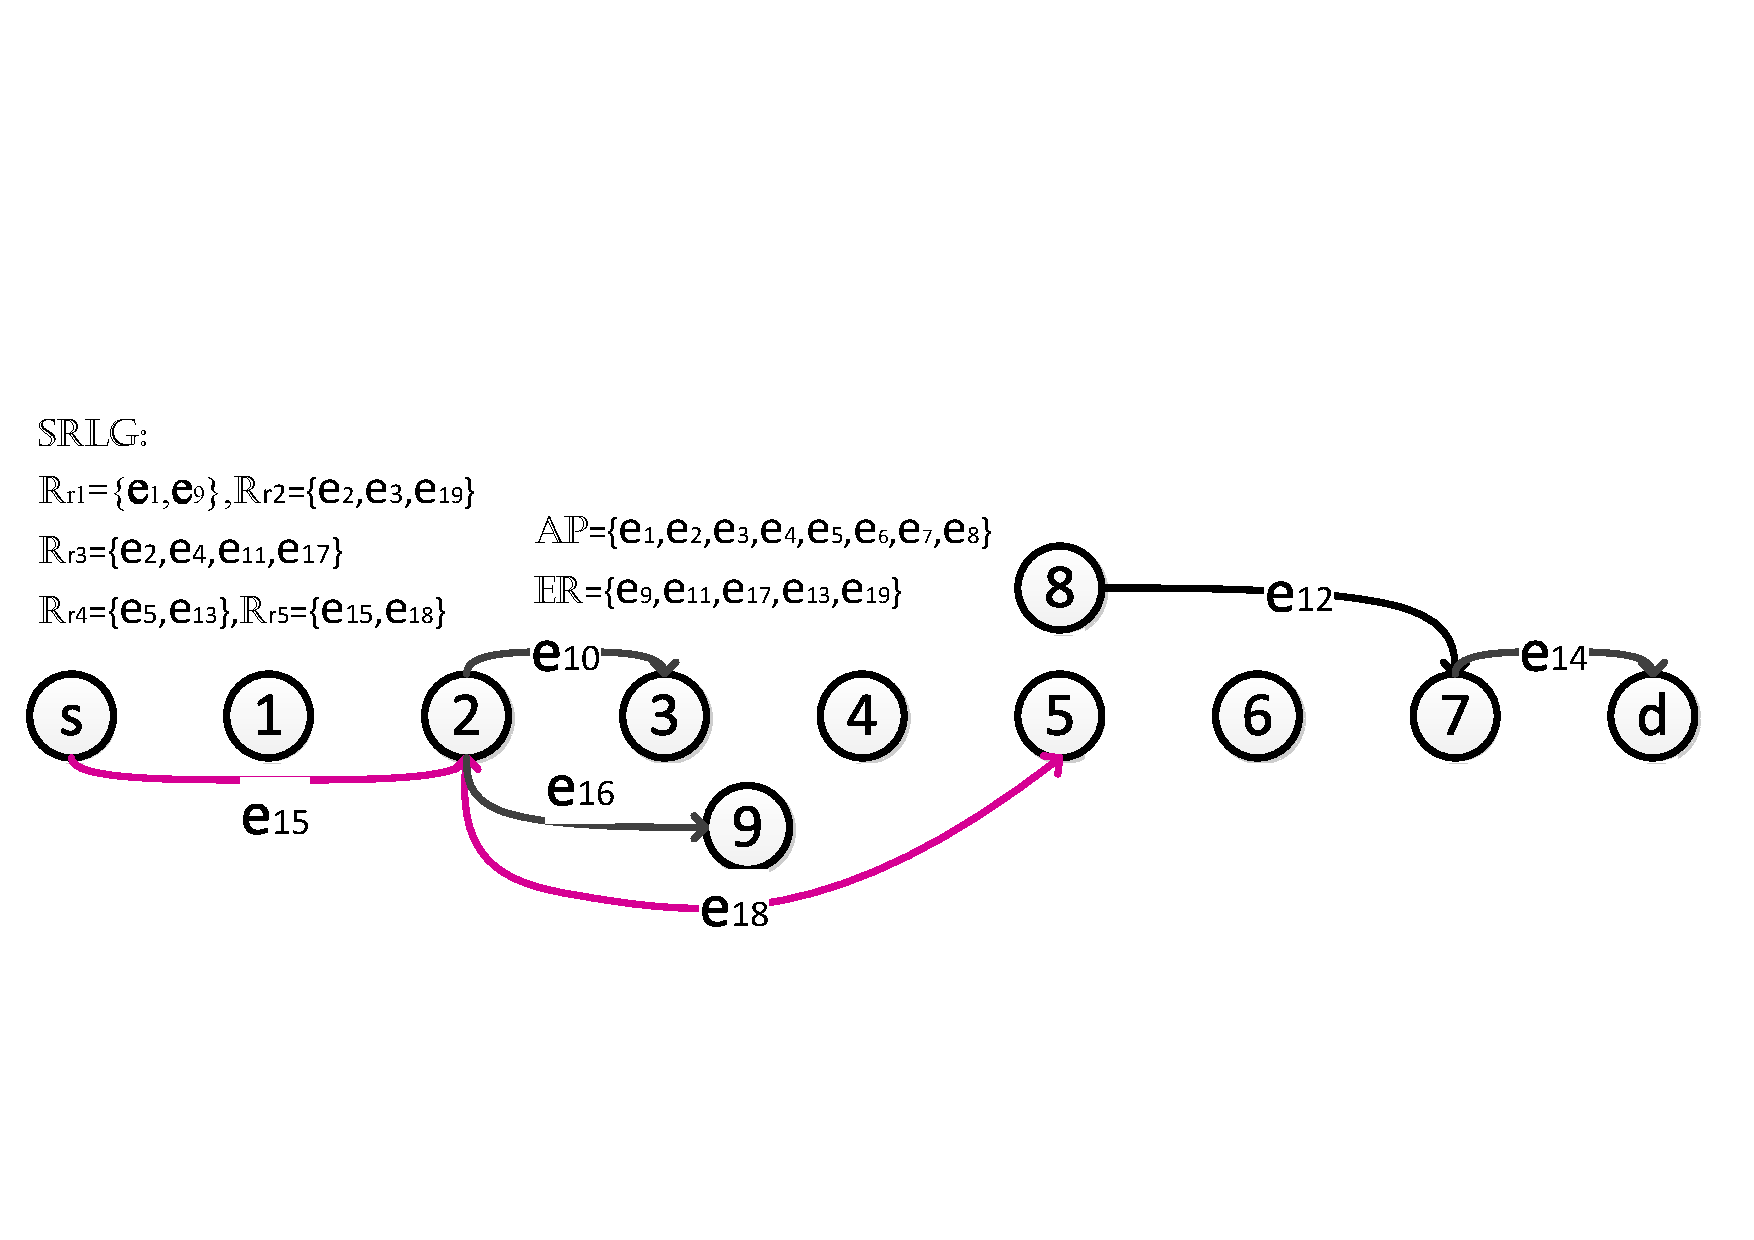
\includegraphics[width=3.5in]{franz/DeletePathGraph}
%\caption{Disconnected graph after deleting the links in $\mathbb{AP}$ and ${\mathbb{ER}}$.}
%\label{fig:DeletePathGraph}
%\end{minipage}
%\end{figure*}

%
%\begin{figure}[tp]
%  \centering
%  % Requires \usepackage{graphicx}
%  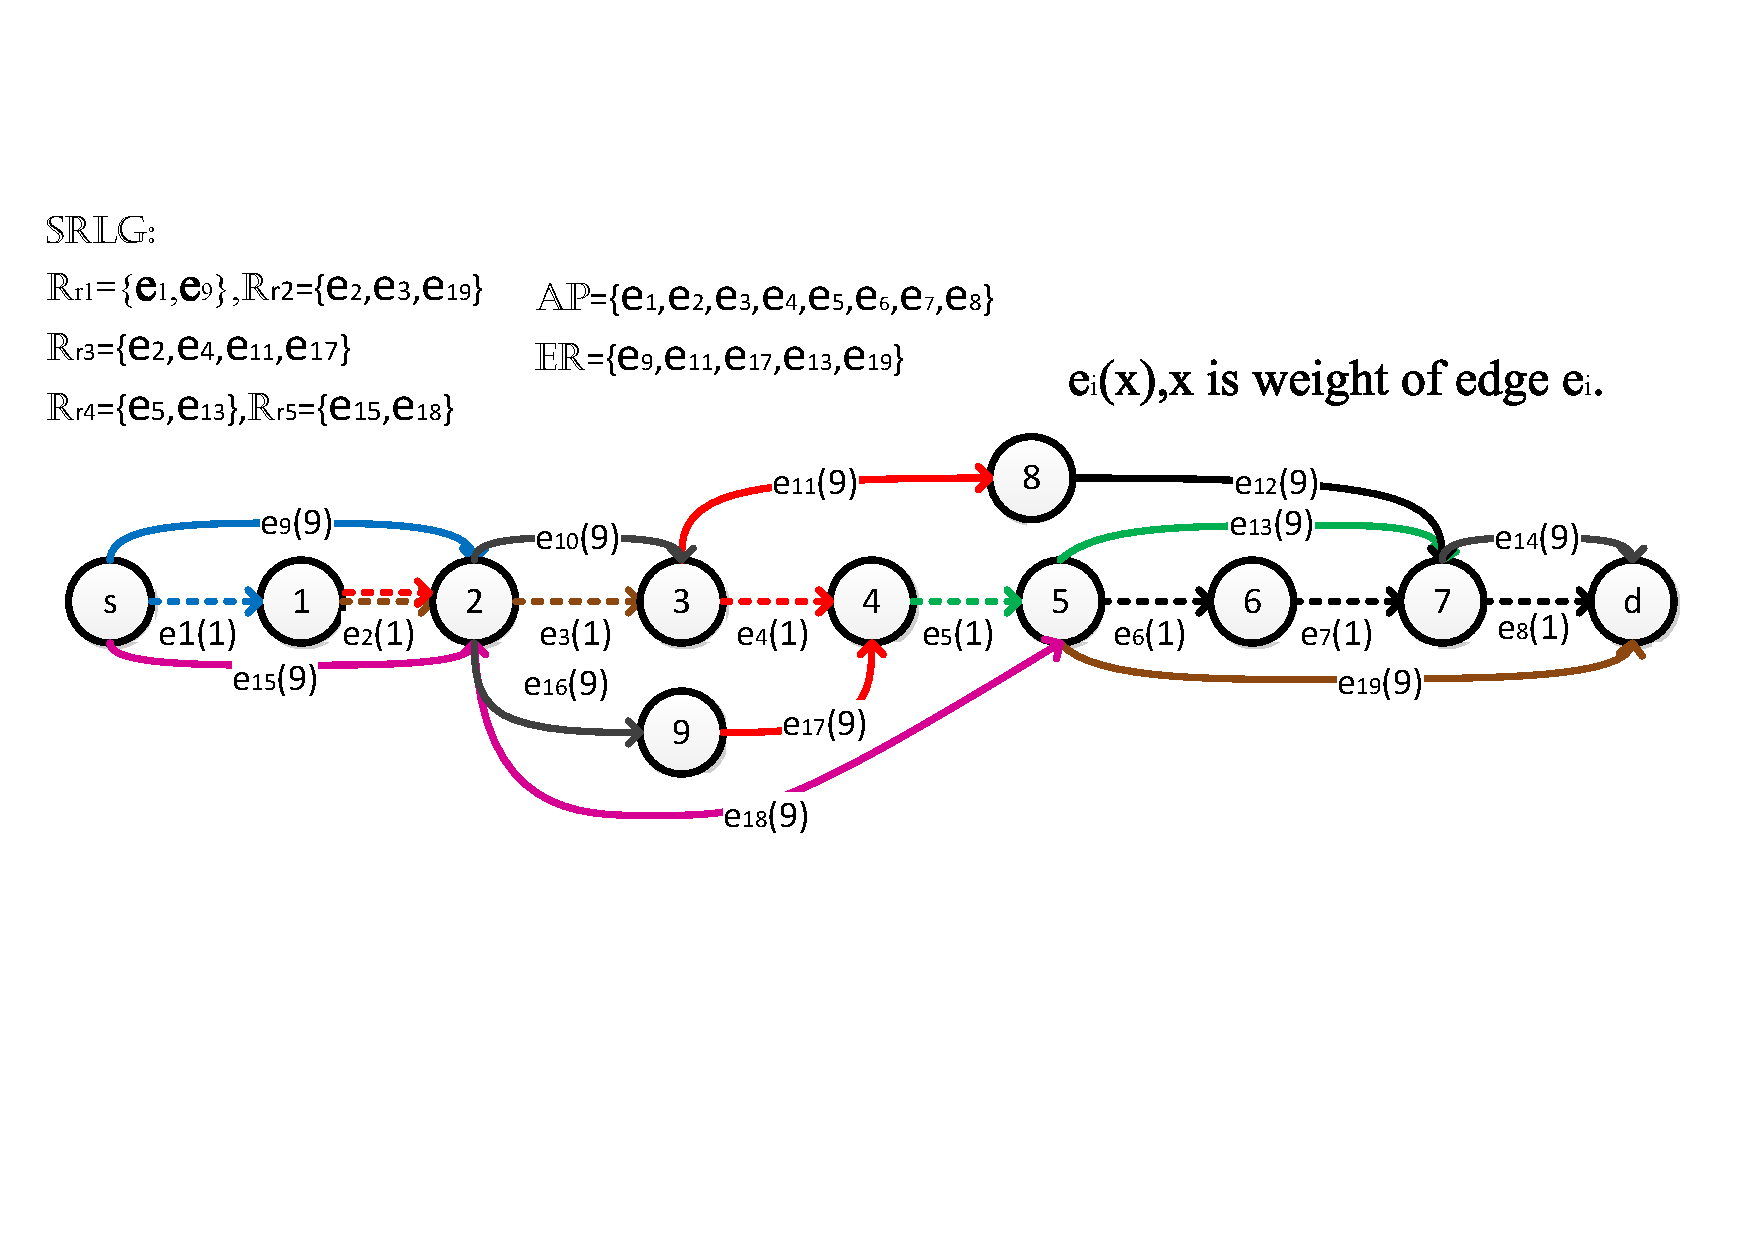
\includegraphics[width=3.6in]{franz/InitialGraph}
%  \caption{$\mathbb{AP}=\{e_1,e_2,e_3,e_4,e_5,e_6,e_7,e_8\}$, $\mathbb{\mathbb{ER}}=\{e_9,e_{11},e_{17},e_{13},e_{19}\}$. SRLGs:$\mathbb{R}_{r_1}=\{e_1,e_9\}$,$\mathbb{R}_{r_2}=\{e_2,e_3,e_{19}\}$,$\mathbb{R}_{r_3}=\{e_2,e_4,e_{11},e_{17}\}$,$\mathbb{R}_{r_4}=\{e_5,e_{13}\}$,$\mathbb{R}_{r_5}=\{e_{15},e_{18}\}$}\label{fig:Initial Graph}
%\end{figure}
%\begin{figure}[tp]
%  \centering
%  % Requires \usepackage{graphicx}
%  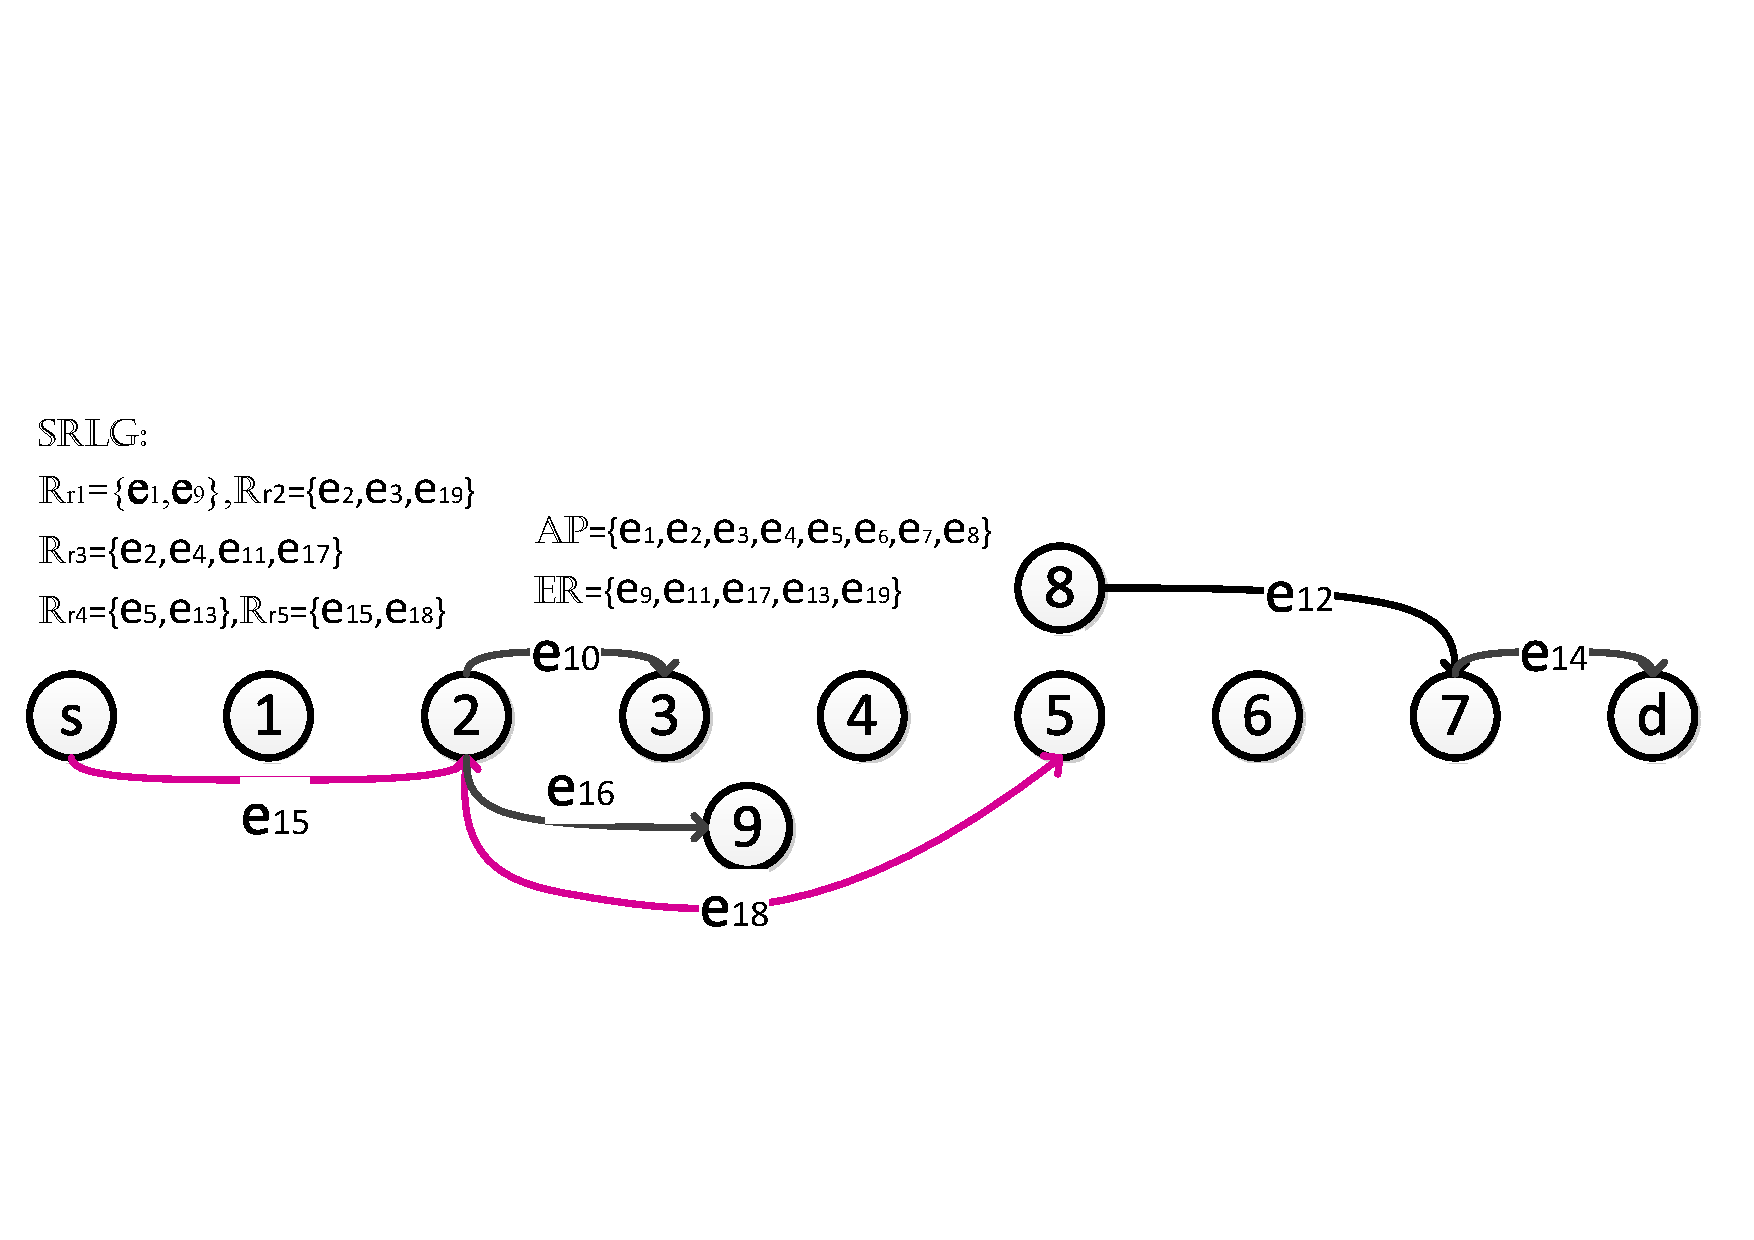
\includegraphics[width=3.4in]{franz/DeletePathGraph}
%  \caption{Disconnected graph after deleting the links in $\mathbb{AP}$ and ${\mathbb{ER}}$.}
%  \label{fig:DeletePathGraph}
%\end{figure}

\begin{figure*}[tp]
  \centering
  % Requires \usepackage{graphicx}
  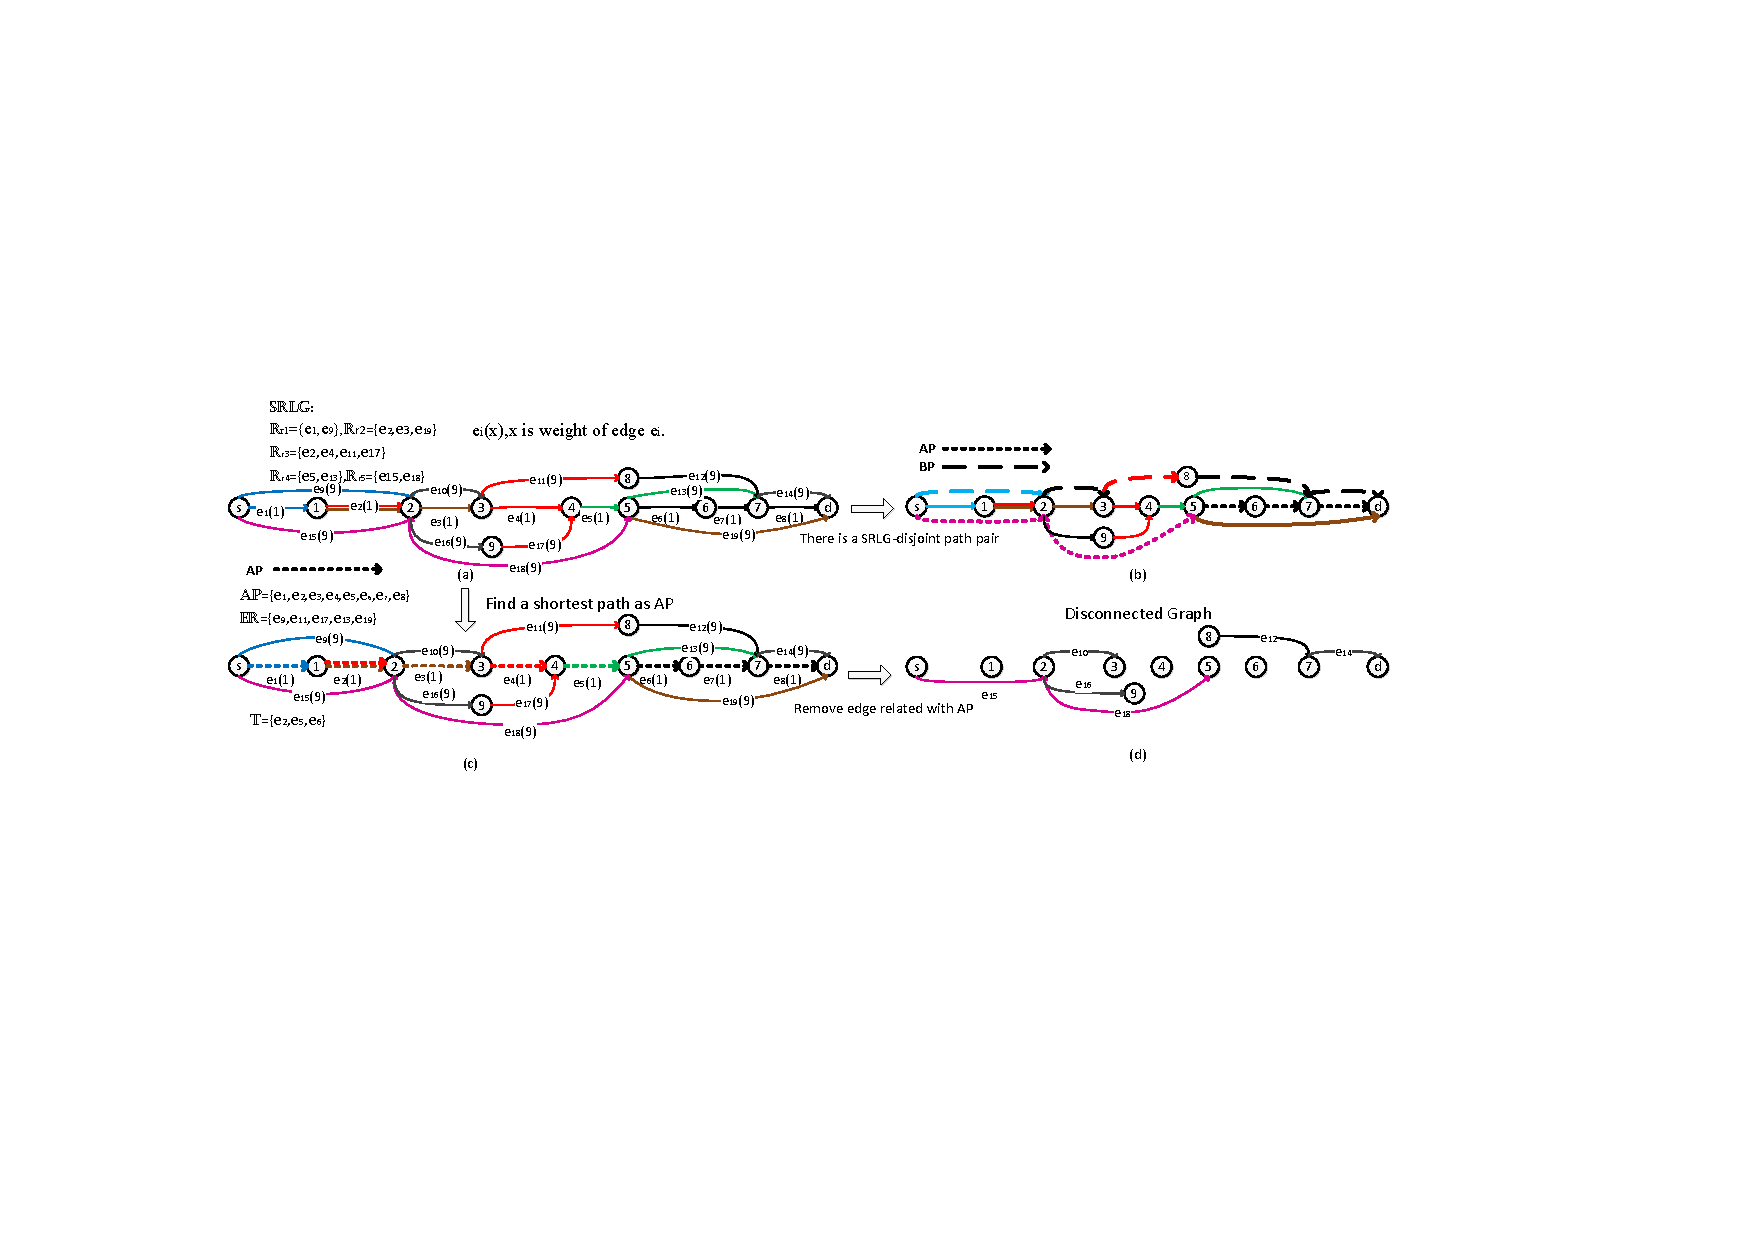
\includegraphics[width=7.2in]{franz/CompositeGraph}
  \caption{(a) A graph with five SRLGs: $\mathbb{R}_{r_1}=\{e_1,e_9\}$,$\mathbb{R}_{r_2}=\{e_2,e_3,e_{19}\}$,$\mathbb{R}_{r_3}=\{e_2,e_4,e_{11},e_{17}\}$,$\mathbb{R}_{r_4}=\{e_5,e_{13}\}$,$\mathbb{R}_{r_5}=\{e_{15},e_{18}\}$. (b)AP and BP in the graph. (c) The shortest weight path AP in the graph. $\mathbb{AP}=\{e_1,e_2,e_3,e_4,e_5,e_6,e_7,e_8\}$, $\mathbb{\mathbb{ER}}=\{e_9,e_{11},e_{17},e_{13},e_{19}\}$. (d)  Graph after deleting the links in $\mathbb{AP}$ and ${\mathbb{ER}}$. }
  \label{fig:CompositeGraph}
\end{figure*}


\subsection{Problem analysis}
\label{sec:NPC proof}
\begin{theorem}
\label{le:lemma1}
    The Min-Min SRLG-disjoint path problem is NP-complete.
\end{theorem}

Proof: Due to the limited space, the proof is omitted.
%
%\subsection{Problem analysis}
%\label{sec:NPC proof}
%\begin{theorem}
%\label{le:lemma1}
%    The Min-Min SRLG-disjoint path problem is NP-complete.
%\end{theorem}
%
%\begin{proof}
%\revtao{
%According to \cite{bhatia2006finding}, the Min-Min link-disjoint path problem is NP-complete.  It is a sub-problem of Min-Min SRLG-disjoint path problem. Denoting the complexity of our Min-Min SRLG-disjoint path problem as C(A), we have NP-complete$\leq$C(A).}
%
%\revtao{
%For proofing complexity of Min-Min SRLG-disjoint path problem less or equal to NPC, we firstly supposed a problem B (denoted as the complexity as C(B)) of finding two SRLG-disjoint paths with the minimum path weight less than or equal to M (M is more than zero integer number). Min-Min SRLG-disjoint routing problem A is equivalent with problem B. We know M must more than zero and less than $\sum\limits_{e_i\in \mathbb{E}}w_{e_i}$. For example, we suppose $0\leq M\leq 10$ and m=6 is optimal solution, through classical binary search method with time complexity O(log(n)) as shown in Fig.\ref{fig:binarySearch}, we obtain two SRLG-disjoint paths with the minimum path optimal weight is m, Therefore problem A equivalent with problem B.}
%
%\revtao{We supposed a program X that when input the problem B if the problem B do not have solution, the program X instantly halt, otherwise program X continue executing and obtaining the problem B's solution, therefore problem B can be reducible to the NP-hard halting problem. Therefore C(B)$\leq$NP-hard}
%
%\revtao{Moreover, given any two paths, it is easy (in polynomial time) to identify whether these two paths are SRLG-disjoint paths and satisfy that the minimum path weight is less than or equal to M, so that C(B)$\leq$NP-complete. As B's complexity is equal to A, we have C(A)=C(B)$\leq$NP-complete. Therefore, A=NP-complete.}
%\end{proof}
%\begin{figure}[tp]
%  \centering
%  % Requires \usepackage{graphicx}
%  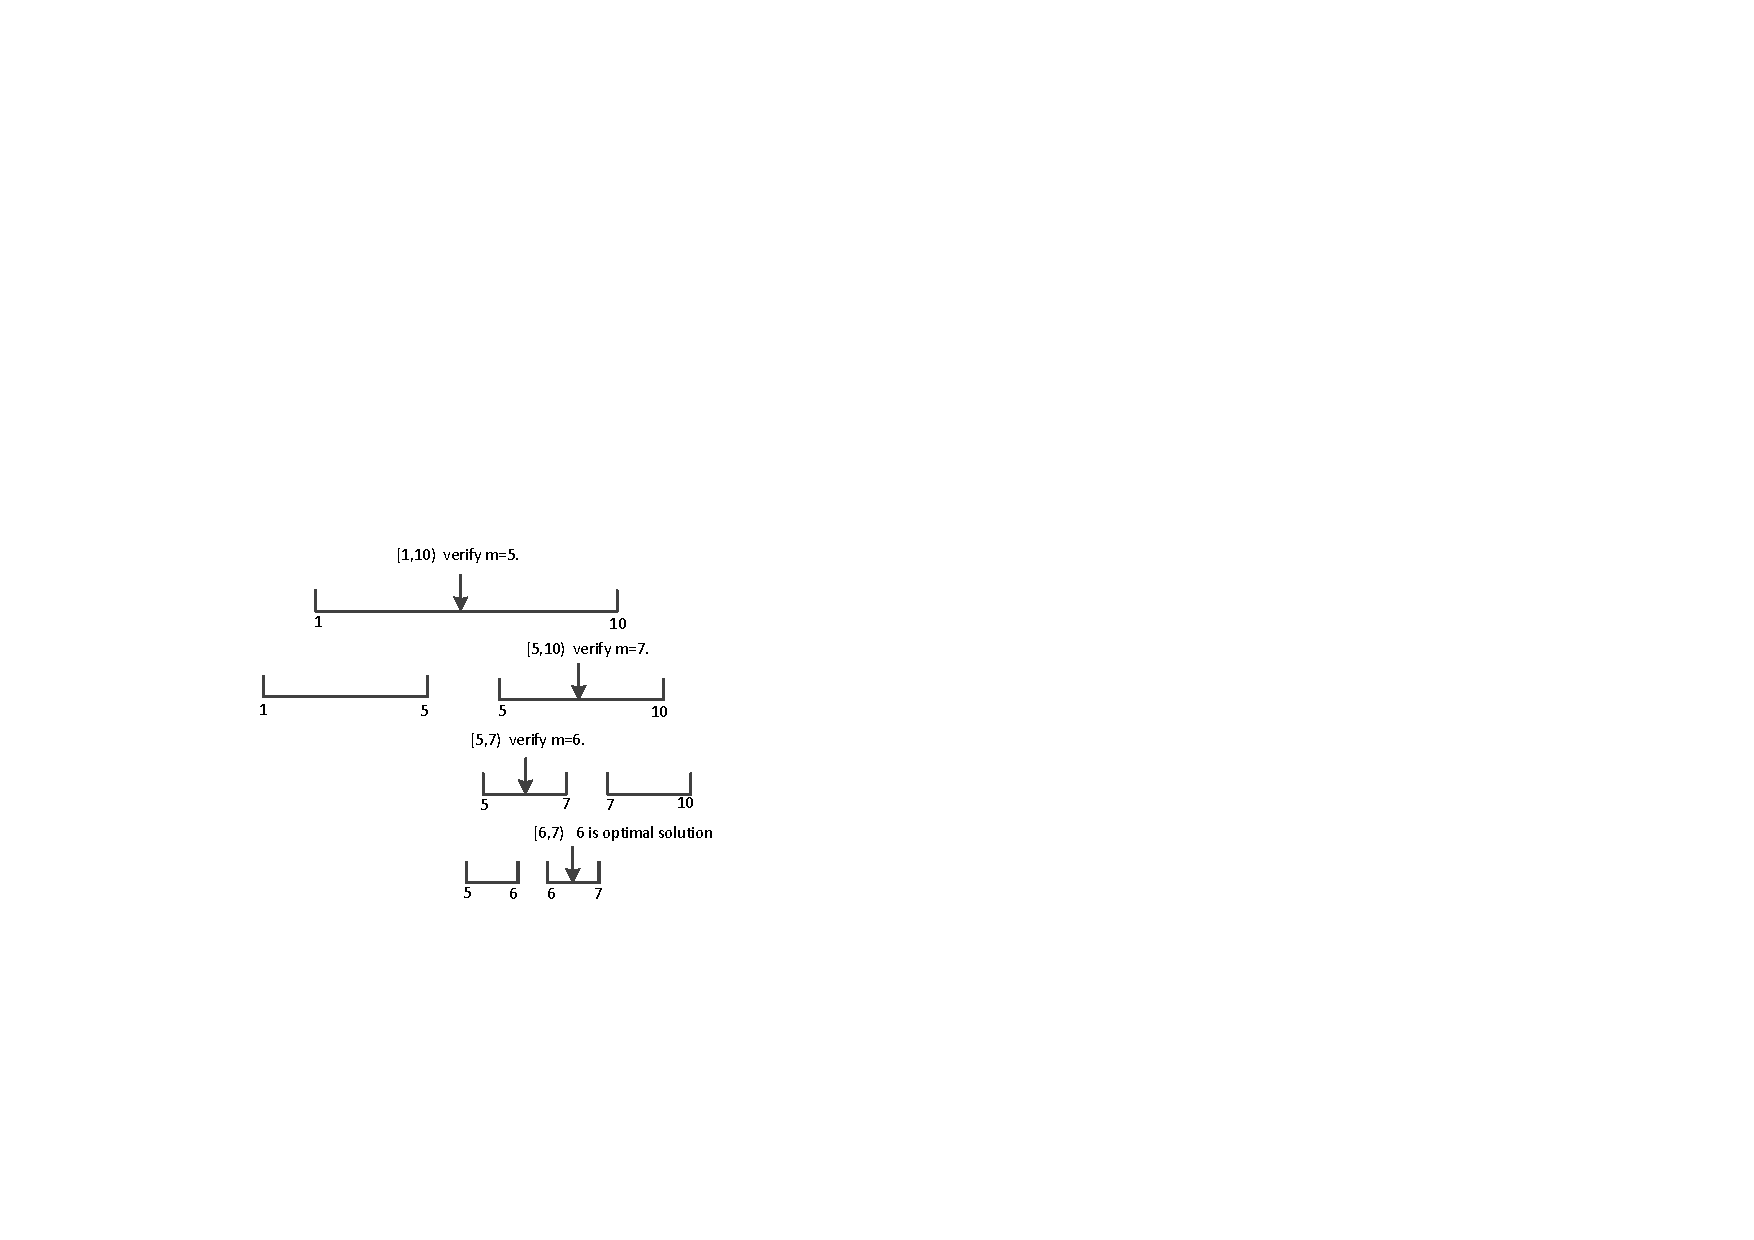
\includegraphics[width=3.0in]{franz/binarySearch}
%  \caption{Request optimal solution M through Binary search method }
%  \label{fig:binarySearch}
%\end{figure}
